\documentclass{article}
\usepackage{tikz}

\begin{document}

drawing

\begin{tikzpicture}
    \draw (0,0) -- (30:1);
    \draw[red] (1,0) -- (2,1);
    \coordinate (S) at (0,1);
    \draw[blue] (S) -- (1,1);
\end{tikzpicture}

\begin{tikzpicture}
    \coordinate (S) at (2,2);
    \draw[gray] (-1,2) -- (S);
    \draw[gray] (2,-1) -- (S);
    \draw[red] (0,0) -- (0,0 -| S);
    \draw[blue] (0,0) -- (0,0 |- S);
\end{tikzpicture}

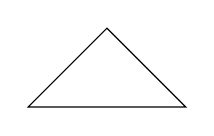
\begin{tikzpicture}
    \draw (0,0) -- (1,1) -- (2,0) -- cycle;
\end{tikzpicture}

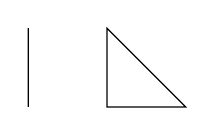
\begin{tikzpicture}
    \draw (0,0) -- (0,1)
    (1,0) -- (1,1) -- (2,0) -- cycle;
\end{tikzpicture}

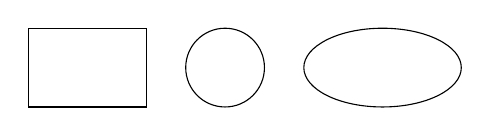
\begin{tikzpicture}
    \draw (0,0) rectangle (1.5,1);
    \draw (2.5,0.5) circle [radius=0.5];
    \draw (4.5,0.5) ellipse
    [x radius=1,y radius=0.5];
\end{tikzpicture}

\begin{tikzpicture}
    \draw (0,0) |- (1,1);
    \draw (1,0) -| (2,1);
    \draw (4,0) arc (0:135:1);
    \draw (6,0) arc (0:135:1 and 0.5);
\end{tikzpicture}

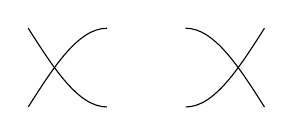
\begin{tikzpicture}
    \draw (0,0) sin (1,1);
    \draw (0,1) sin (1,0);
    \draw (2,1) cos (3,0);
    \draw (2,0) cos (3,1);
\end{tikzpicture}

\begin{tikzpicture}
    \draw (0,0) parabola (1,2);
    \draw (2,0) parabola
    bend (2.25,-0.25) (3,2);
    \draw (4,0) parabola
    bend (4.75,2.25) (5,2);
\end{tikzpicture}

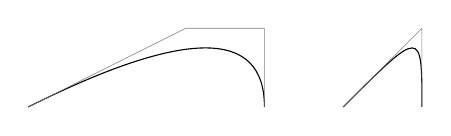
\begin{tikzpicture}
    \draw (0,0) .. controls
    (2,1) and (3,1) .. (3,0);
    \draw (4,0) .. controls
    (5,1) .. (5,0);
    \draw[help lines] (0,0)
    -- (2,1) -- (3,1) -- (3,0)
    (4,0) -- (5,1) -- (5,0);
\end{tikzpicture}

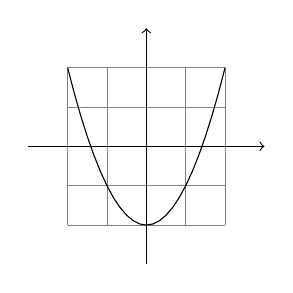
\begin{tikzpicture}
    \draw[help lines,step=0.5]
    (-1,-1) grid (1,1);
    \draw[->] (-1.5,0) -- (1.5,0);
    \draw[->] (0,-1.5) -- (0,1.5);
    \draw[domain=-1:1]
    plot(\x,{\x*\x*2 -1});
\end{tikzpicture}

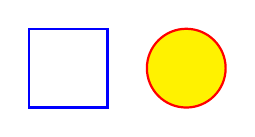
\begin{tikzpicture}[thick]
    \draw[blue] (0,0) rectangle (1,1);
    \filldraw[fill=yellow,draw=red]
    (2,0.5) circle [radius=0.5];
\end{tikzpicture}

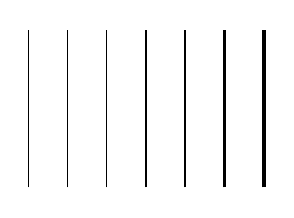
\begin{tikzpicture}
    \draw[ultra thin] (0,0)--(0,2);
    \draw[very thin] (0.5,0)--(0.5,2);
    \draw[thin] (1,0)--(1,2);
    \draw[semithick] (1.5,0)--(1.5,2);
    \draw[thick] (2,0)--(2,2);
    \draw[very thick] (2.5,0)--(2.5,2);
    \draw[ultra thick] (3,0)--(3,2);
\end{tikzpicture}

\begin{tikzpicture}
    \draw[dashed] (0,0) -- (0,2);
    \draw[dotted] (0.5,0) -- (0.5,2);
    \draw[dash dot] (1,0) -- (1,2);
    \draw[dash dot dot] (1.5,0) -- (1.5,2);
    \draw[densely dotted]
    (2,0) -- (3,2) -- (4,0) -- cycle;
\end{tikzpicture}

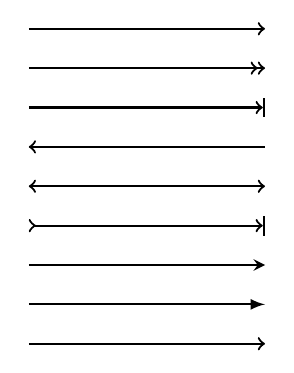
\begin{tikzpicture}[thick]
    \draw[->] (0,4) -- (3,4);
    \draw[->>] (0,3.5) -- (3,3.5);
    \draw[->|] (0,3) -- (3,3);
    \draw[<-] (0,2.5) -- (3,2.5);
    \draw[<->] (0,2) -- (3,2);
    \draw[>->|] (0,1.5) -- (3,1.5);
    \draw[-stealth] (0,1) -- (3,1);
    \draw[-latex] (0,0.5) -- (3,0.5);
    \draw[-to] (0,0) -- (3,0);
\end{tikzpicture}

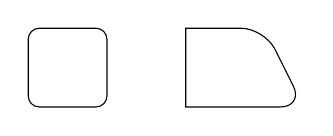
\begin{tikzpicture}
    \draw[rounded corners]
    (0,0) rectangle (1,1);
    \draw (2,0) -- (2,1)
    [rounded corners=.3cm]
    -- (3,1) -- (3.5,0)
    [sharp corners] -- cycle;
\end{tikzpicture}

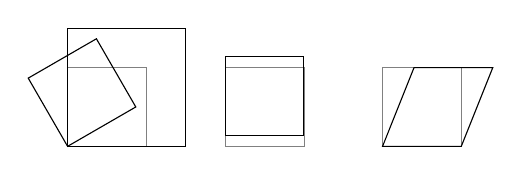
\begin{tikzpicture}
    \draw[help lines](0,0) rectangle (1,1);
    \draw[scale=1.5] (0,0) rectangle (1,1);
    \draw[rotate=30] (0,0) rectangle (1,1);
    \draw[help lines](2,0) rectangle (3,1);
    \draw[yshift=4pt](2,0) rectangle (3,1);
    \draw[help lines](4,0) rectangle (5,1);
    \draw[xslant=0.4](4,0) rectangle (5,1);
\end{tikzpicture}

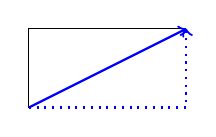
\begin{tikzpicture}
    [myarrow/.style={blue,thick,->}]
    \draw (0,0)--(0,1)--(2,1);
    \draw[myarrow] (0,0)--(2,1);
    \draw[myarrow,dotted]
    (0,0)--(2,0)--(2,1);
\end{tikzpicture}

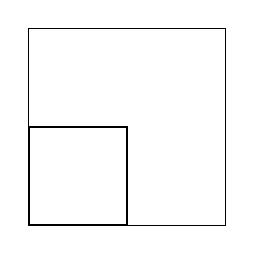
\begin{tikzpicture}
    \draw (0,0) rectangle (2.5, 2.5);
    \begin{scope}[thick,scale=0.5]
    \draw (0,0) rectangle (2.5, 2.5);
    \end{scope}
\end{tikzpicture}

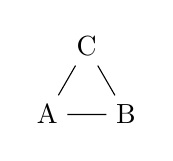
\begin{tikzpicture}
    \node (A) at (0,0) {A};
    \node (B) at (1,0) {B};
    \node (C) at (60:1) {C};
    \draw (A) -- (B) -- (C) -- (A);
\end{tikzpicture}

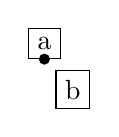
\begin{tikzpicture}
    \coordinate (A) at (1,1);
    \fill (A) circle[radius=2pt];
    \node[draw,anchor=south] at (A) {a};
    \node[draw,below right=4pt] at (A) {b};
\end{tikzpicture}

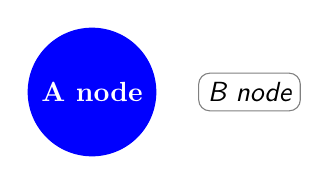
\begin{tikzpicture}
    \node[circle,fill=blue,text=white,
    node font={\bfseries}]
    (A) at (0,0) {A node};
    \node[rectangle,rounded corners,
    draw=gray,
    node font={\sffamily\slshape}]
    (B) at (2,0) {B node};
\end{tikzpicture}

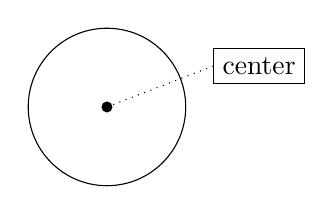
\begin{tikzpicture}
    \draw (0,0) circle[radius=1];
    \fill (0,0) circle[radius=2pt];
    \node[draw] (P) at (15:2) {center};
    \draw[dotted] (0,0) -- (P.west);
\end{tikzpicture}

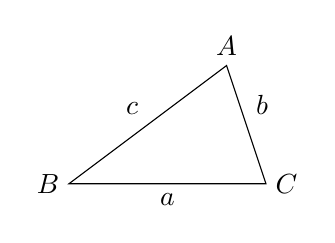
\begin{tikzpicture}
    \draw (2,1.5) node[above] {$A$}
    -- node[above left] {$c$}
    (0,0) node[left] {$B$}
    -- node[below] {$a$}
    (2.5,0) node[right] {$C$}
    -- node[above right] {$b$}
    cycle;
\end{tikzpicture}

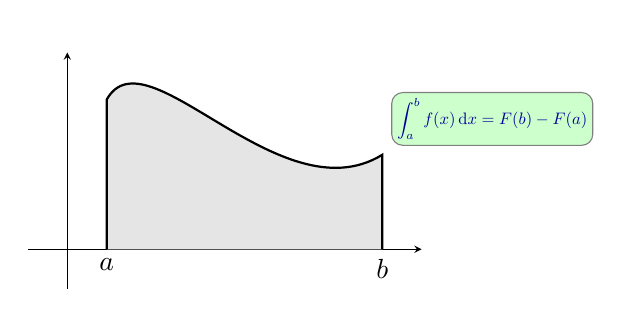
\begin{tikzpicture}
    \draw[-stealth,line width=0.2pt] (-0.5,0) -- (4.5,0);
    \draw[-stealth,line width=0.2pt] (0,-0.5) -- (0,2.5);
    \coordinate (a) at (0.5,1.9);
    \coordinate (b) at (4,1.2);
    \node[below] (a0) at (a |- 0,0) {$a$};
    \node[below] (b0) at (b |- 0,0) {$b$};
    \filldraw[fill=gray!20,draw,thick]
    (a0) -- (a) .. controls (1,2.8) and (2.7,0.4) .. (b) -- (b0) -- cycle;
    \node[above right,outer sep=0.2cm, rounded corners,
    fill=green!20,draw=gray,text=blue!60!black,scale=0.6]
    at (b) {$\displaystyle \int_a^b {f(x)\,\mathrm{d}x} = F(b) - F(a)$};
\end{tikzpicture}

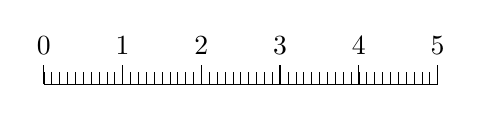
\begin{tikzpicture}
    \draw (0,0)--(5,0);
    \foreach \i in {0.0,0.1,...,5.0}
    {\draw[very thin]
    (\i,0)--(\i,0.15);}
    \foreach \I in {0,1,2,3,4,5}
    {\draw (\I,0)--(\I,0.25)
    node[above] {\I};}
\end{tikzpicture}

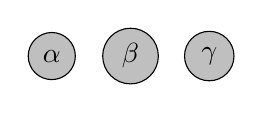
\begin{tikzpicture}
    \foreach \n/\t in
    {0/\alpha,1/\beta,2/\gamma}
    {\node[circle,fill=lightgray,draw]
    at (\n,0) {$\t$};}
\end{tikzpicture}

\end{document}

